% !TEX root = ../../report.tex
\clearpage
\section{Experimental Plan}

%We can sometimes evaluate how well the recommender achieves its overall goals.
%For example, we can check an e-commerce website revenue with and without the
%recommender system and thereby estimate the value of the system to the website.

Section \ref{evaluation} covers a wide range of evaluation metrics that
measure different properties of the recommender system. This section will cover
our experimental plan, starting off by looking at the goals for our experiments.
The remaining parts of the section will describe the datasets used for evaluation,
our evaluation methodology and our evaluation metrics of choice.
The section will also describe the datasets used for evaluation, our evaluation methodology

We have the following goals for our experiment:

\begin{itemize}
	\item Does our proposed implicit rating methods improve the recommendation quality over
	binary preference data?
	\item Compare the different implicit rating functions.
	\item Select the best combination of methods for the SoBazaar recommender system.
\end{itemize}

\marginpar{Supervisors: Any suggestions?}
\marginpar{TODO: Discussion on how}

Then the question is, how can we determine whether a method is better than another. The
main reasons for implementing a recommender system is the desire to improve user
satisfaction and to increase the economic success of a platform. Although both goals
are interrelated they may be competing in some scenarios. The user might be more interested
in purchasing the products with the best price-performance ratio, while the \emph{owners}
are more interested in showing the products that lead to the highest revenue for the
business. For this purpose, a commercial recommender could/should consider implementing
a reward attribute for items that show how much the company profits from its sale. This
information can then e.g. be used in a combination the recommendation list of the recommender
to produce the final recommendations.

\begin{figure}[H]
		\centering
	  	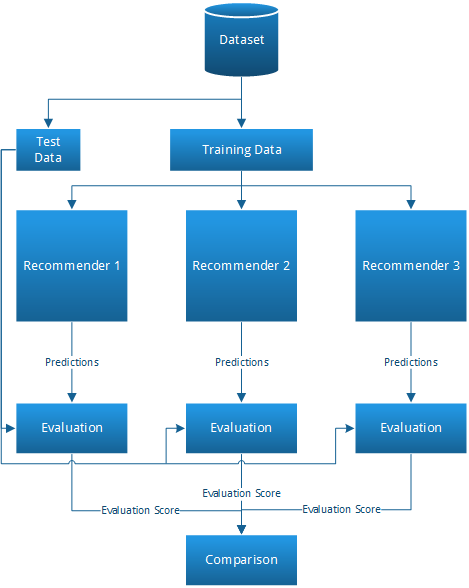
\includegraphics[height=0.65\linewidth]{image/evaluationpipeline.png}
		\caption[A Traditional Evaluation Pipeline]{A traditional evaluation pipeline for evaluating recommender systems}
		\label{figure:evaluationpipeline}
\end{figure}

In order to further specify our goals we therefore have to take a closer look at the recommender's task,
its interface and the available data. The most typical task for a e-commerce recommender system is to determine an order of items, often with the purpose of creating a top-k list of items that is shown in a sidebar or on a
dedicated page.

\begin{figure}[H]
		\centering
		\begin{minipage}{.45\linewidth}
	  		
\includegraphics[height=1.2\linewidth]{image/SoBazaarfeed2.png}
		\end{minipage}
		\begin{minipage}{.45\linewidth}
			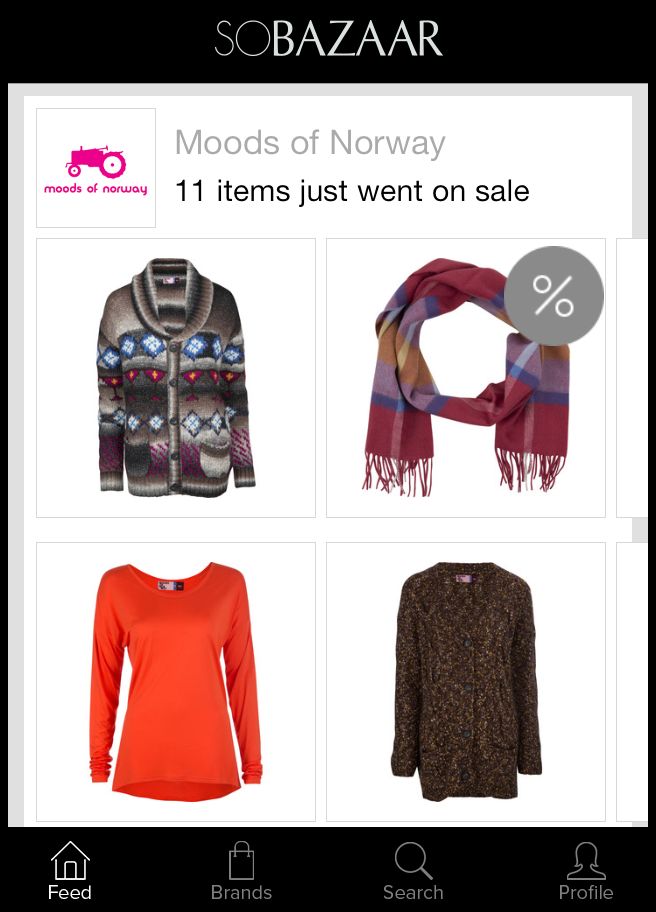
\includegraphics[height=1.2\linewidth]{image/SoBazaarsale.png} 
		\end{minipage}
		\caption[SoBazaar news feed - version 0.5.1]{SoBazaar news feed}
		\label{figure:SoBazaarfeed}
\end{figure}


The above figure shows the SoBazaar feed. Recommendations are likely to be shown in a similar fashion, but instead as \emph{recommended for you}. The interface currently let you scroll sideways over up to 20 items.

Ultimately, the goal of the experiment is to evaluate and measure the properties
of the system, which we have identified as the most important for the systems success,
and select the method that performs the best overall with respect to these properties.

\subsection{Selecting datasets for evaluation}

In addition to evaluate the methods on the SoBazaar dataset we want to make sure that our
solution generalizes beyond our experimental dataset, in accordance to the general guidelines
for experimental studies \cite{Shani2011}. The data used for offline evaluation should match
as closely as possible the data we expect the recommender system to face when it is
deployed \cite{Gunawardana2009}. When selecting datasets for evaluation we focused on the
following dataset properties:

\begin{itemize}
	\item Size of dataset: Preferable as close as possible to SoBazaar (6 months from now)
	in terms of number of ratings, users and items.
	\item Different types of user feedback: Preferable different types of implicit feedback
	such as browsing and buying behavior.
	\item Domain: Preferably a domain as close to possible as the e-commerce domain with respect
	to the importance of factors such as recentness.
	\item Presence of features: To evaluate the hybrid methods.
	\item Timestamps: To evaluate the recentness mapping
\end{itemize}

We were unable to acquire any e-commerce datasets containing user browsing history, purchases etc.
And we therefore had to turn for other domains for datasets...

%The first dataset we chose for evaluation was the MovieLens 1M dataset. The reason for selecting the MovieLens 1M dataset over MovieLens 100K is that the number of users is closer to what we expect the SoBazaar to have after the \emph{official} launch this summer in addition to having user- and item features. The MovieLens dataset can also be seen as a \emph{benchmark} dataset as it is one of the most popular recommender systems dataset used for evaluation in countless articles.

\subsubsection{Book-Crossing Dataset?}

Use implicit feedback as \emph{item-clicked} and explicit ratings greater than 5 as \emph{item-liked}.

\subsection{Simulating user behavior?}

%General statistics and averages
%Interesting findings/properties
%Was cleaning neccesary?
%How was the methods evaluated on the dataset?
%	- x-fold cross validation


%\subsubsection{MovieLens 1M}
%
%As our second dataset we have chosen the MovieLens 1M dataset. The dataset contain 1,000,209 anonymous ratings on approximately 3,706 movies (The readme mentions 3900 movies) made by 6040 users. User features included age, gender, occupation and zipcode, item features include movie genre. Each user included in the dataset have provided a minimum of 20 ratings. The average rating given to movies in the dataset is $3.58$. There are 18 different genres in the dataset, but each movie can have multiple genres assigned to it, of which there are 498 different combinations in the dataset.
%
%\begin{table}[H]
%\centering
%\begin{tabular}{|l|l|}
%\hline
%Male & Female \\ \hline
%4331 & 1709 \\ \hline
%\end{tabular}
%\caption{MovieLens Gender Distribution}
%\end{table}
%
%\begin{table}[H]
%\centering
%\begin{tabular}{|l|l|l|l|l|l|l|}
%\hline
%Under 18 & 18-24 & 25-34 	& 35-44 	& 45-49 & 50-55 & 56+ \\ \hline
%222		 &	1103 &	2096	&	1193	& 550	& 496	& 380 \\ \hline
%\end{tabular}
%\caption{MovieLens 1M Age Group Distribution}
%\end{table}
%
%\begin{table}[H]
%\centering
%\begin{tabular}{|l|l|}
%\hline
%Other/not specified  & 711  \\ \hline
%Academic/Educator  & 528  \\ \hline
%Artist  & 267 \\ \hline
%Clerical/Admin & 173 \\ \hline
%College/Grad student  & 759 \\ \hline
%Customer service & 112 \\ \hline
%Doctor/Health care & 236 \\ \hline
%Executive/Managerial & 679 \\ \hline
%Farmer & 17 \\ \hline
%Homemaker & 92 \\ \hline
%K-12 student & 195 \\ \hline
%Lawyer & 129 \\ \hline
%Programmer & 388 \\ \hline
%Retired & 142 \\ \hline
%Sales/Marketing & 302 \\ \hline
%Scientist & 144 \\ \hline
%Self-employed & 241 \\ \hline
%Technician/Engineer & 502 \\ \hline
%Tradesman/Craftsman & 70 \\ \hline
%Unemployed & 72 \\ \hline
%Writer & 281 \\ \hline
%\end{tabular}
%\caption{MovieLens 1M Occupation Distribution}
%\end{table}
%
%As the sparsity of this dataset is fairly low (95.53164), we decided to evaluate this dataset using the holdout method. As the dataset include time-stamps we split the dataset based on time, meaning that all ratings given before a given time will be used to train the model and all ratings given after this point will be used as a testset. We set aside the last 25\% ratings for evaluation and train the model using the remaining 75\%.

\subsubsection{The SoBazaar Dataset}

The SoBazaar dataset is smallest and sparsest of our datasets used for evaluation.
The dataset contain ratings 15,252 given by 1,235 users to 3,386 items.
We also have access to semi-structured product information collected/crawled from
the online retailers for \emph{some} items. In addition user data from the users
can also be downloaded from Facebook.

Having such a small and sparse dataset has several implications. Firstly we have
to avoid \emph{wishful thinking} as we have very thin data, meaning that we cannot
rely on getting reliable results. Secondly, our evaluation methodology must be
\emph{tailored} for small sparse datasets. When using cross-validation the number
of folds depends on the size of the dataset. For large datasets, even 3-fold Cross
Validation will be quite accurate, while for very sparse datasets, we may have to
use leave-one-out in order to train on as many examples as possible. The advantages
of using a large number of folds is that the bias of the true error rate estimators
will be small (the estimator will be very accurate), with the disadvantages being that
the variance of the true error rate estimator will be large in addition to increased
computation time. To exemplify this we ran a small experiment on the SoBazaar data using
IBCF, with $k-NN=3$, experimenting with different $K$-fold values:

\begin{table}[H]
\centering
\begin{tabular}{l l l l l }
\toprule
K-fold & 	$min_{RMSE}$ 	&	$max_{RMSE}$ 	& Average 	& Variance 					\\ \midrule
3	   & 	0.783 			& 	0.789 			& 0.785 	& $8.730 \times 10^{-6}$	\\ 
5	   & 	0.759			& 	0.802 			& 0.781 	& $3.363 \times 10^{-4}$ 	\\ 
8	   & 	0.740			& 	0.781			& 0.758 	& $1.656 \times 10^{-4}$ 	\\ 
10	   & 	0.718 			& 	1.026			& 0.810  	& 0.0125					\\
\bottomrule
\end{tabular}
\caption{Evaluation results from experimenting with different k-fold splits on the SoBazaar dataset}
\end{table}

\marginpar{TODO: This table is not really necessary to include...}

When increasing the number of folds we could see that it was unable to generate
any recommendations at all for some folds, or getting really poor results, meaning
that we get some difficult splits. E.g. when using 30 folds, IBCF was unable to
provide any recommendations for 8 folds out of 30. By using more than 10 folds
it is increasingly likely that we end up with a few or more \emph{unrecommendable}
instances in the test set, yielding no test result. Based on these results,
and the general consensus that more folds are better for small datasets we
believe that using between $5-10$-folds would be a good choice for model validation.
Another alternative well suited for sparse datasets is the \emph{all but one} or the
\emph{leave one out} method, in which we remove one rating from the test users
and try to predict the hidden rating.

Another important concern is whether or not to take the timestamps into consideration,
which directly speaks against the use of cross-validation, as we wish to use the past
interactions to predict future actions. When using the \emph{leave one out} method one
could e.g. select a predetermined set of test users based on some criteria and remove
their latest rating and try to predict it and repeat the process any number of times.
This is particularly relevance as our implicit mapping function takes recency into account.


\subsubsection{Overview of the Datasets}

Table \ref{table:datasets} shows an overview of the datasets used for evaluation.

%TODO - What else is interesting to know? Rating scale, average number of ratings per user, number of cold start users...
%TODO - % of users with less than 5 ratings for both datasets

\begin{table}[H]
    \centering
    \begin{tabular}{l l l l l l }
    \toprule
	Dataset			& 	Ratings 	& 	Users	& 	Items 	& 	Sparsity	& Rating Scale 				\\ \midrule
	SoBazaar 		& 	27,873  	& 	1,511	&	5855	&	99.69657	& Implicit Ratings(1-5)		\\ 
	%Movielens 1M	& 	1,000,029   &	6040 	&	3706	&	95.53164	& Explicit (1-5)			\\ 
	Dataset 2 		& 	-  			& 	-		&	-		&	-			&							\\
	\bottomrule
    \end{tabular}
    \caption [Overview of the datasets used for evaluation]{Overview of the datasets used for evaluation}
    \label{table:datasets}
\end{table}

\subsection{Simulating the Cold-Start Problem}

To simulate the cold-start problem and evaluate how well our the different
methods tackle the different cold-start situations we used the following
evaluation methodology. As mentioned in Section \ref{sec:cold-start-eval} there is
no common framework for assessing the cold-start performance of recommender systems.
Our goal is to come up with \emph{comprehensive} framework to assess the cold-start
performance of our recommender systems. The following inputs changes the dataset over time:

\begin{itemize}
	\item 	Existing users watch new items in the catalogue
	\item	New users join the system and view their first item
	\item	New items are added to the catalogue
\end{itemize}

The first input source has the effect of increasing the dataset density, the average user
profile length, and the average number of views per item. The second input factor has
the effect of decreasing both the dataset density and the average user profile length,
as the new users that join the system have interacted with only a few items. Similarly, the third input
factor has the effect of decreasing both the dataset density and the average number of
views per item.

To simulate the cold-start user problem we propose splitting the users into two disjoint
sets, similarly as in \cite{Stern2009, Lam2008}, using 90\% of the users for training and
setting aside the remaining 10\% for evaluation. We then train the model with e.g. 5, 15,
25 and 35 ratings and predict the remaining values. Alternatively one could train the model
using e.g. 25\% and 75\% of each test users ratings. Similarly, to simulate the cold-start
item problem we again split the items into two disjoint sets, using 90\% of the items
for training and the remaining 10\% for evaluation.  We then train the model with
e.g. 20, 40, 60 and 80 ratings and predict the remaining values. The selection criteria
for test items and users can differ from dataset to dataset. E.g. in \cite{Rashid2002, Rashid2008}
the authors selected a subset of the users with more than 200 ratings, but you can not
expect 10\% all the users for all datasets to have provided 200 ratings, so this number
might be lowered if necessary. The implications of removing the top 10\% of the
raters from the SoBazaar dataset is fairly large as they stand for a large portion
of the few ratings we have.

To evaluate the cold-start system performance we use the same method as described
in ~\cite{Agarwal2009} where the authors propose using a 75:25 training/test split,
where we at random draw e.g. 35\%, 50\% and then finally use all (75\%) of the
ratings in the training set and predict the remaining 25\%.

\marginpar{TODO: Add some justification...}

%TODO - How is this implemented on the SoBazaar data?

For the SoBazaar dataset we select 10\% of the users as test users, for a user to be
selected as a test user, the user must have provided at least 20 ratings. The test user are drawn
at random from the eligible candidates. We then train
the model using 10\%, 40\% and 75\% of their ratings and try to predict their remaining ratings.
The reason for choosing percentages over hard limits is due to the fact that the ratings are
distributed unevenly among the users. As we have a very low number of ratings and a large item collection we had to use
only 5\% of the items as test items, where each test item have been rated by atleast 15 users.
We train the model using 10\%, 40\% and 75\% of their ratings and try to predict their remaining
ratings. As we have access time timestamps, we split the users and items based on timestamp.
E.g. for the 10\% user split we train the model with their initial ratings and try to predict
their following ratings. To evaluate the cold-start system performance we split the dataset in a test
and training set using 20\% of the ratings for testing and then train the model
using 40\%, 60\% and 80\% of the ratings for training. It is important to note that
this process should be repeated multiple times, as the chance of getting an
\emph{unfortunate} split is highly probable due to the dataset size. For the cold-start
system task we also split the dataset based on timestamps, meaning that the test set consists
of the most recent ratings.

%TODO - How is this implemented on the x dataset?


\subsection{Evaluation Metrics}

%TODO - Discussion of evaluation metrics

%http://www.slideshare.net/gunnar-schroeder

A large variety of metrics have been published, and some of these metrics are highly correlated \cite{Herlocker2004}.
There is little guidance for evaluating recommender systems and choosing metrics. However, there are
some important questions one should ask oneself when selecting evaluation metrics:

\begin{itemize}
	\item Which aspects of the usage scenario and the data influence the choice?
	\item Which metrics are applicable?
	\item What does these metrics express?
	\item What are the differences among them?
	\item Which metric represent our user-case best?
	\item How much do the metrics suffer biases?
\end{itemize}

It is safe to assume that the users are more interested in the top ranked items, than rating
predictions for the entire item collection. Evaluation of top-k recommendations suggests a
classification or ranking task, evaluation should therefore focus on classification or ranking metrics.

\begin{figure}[H]
  \centering
  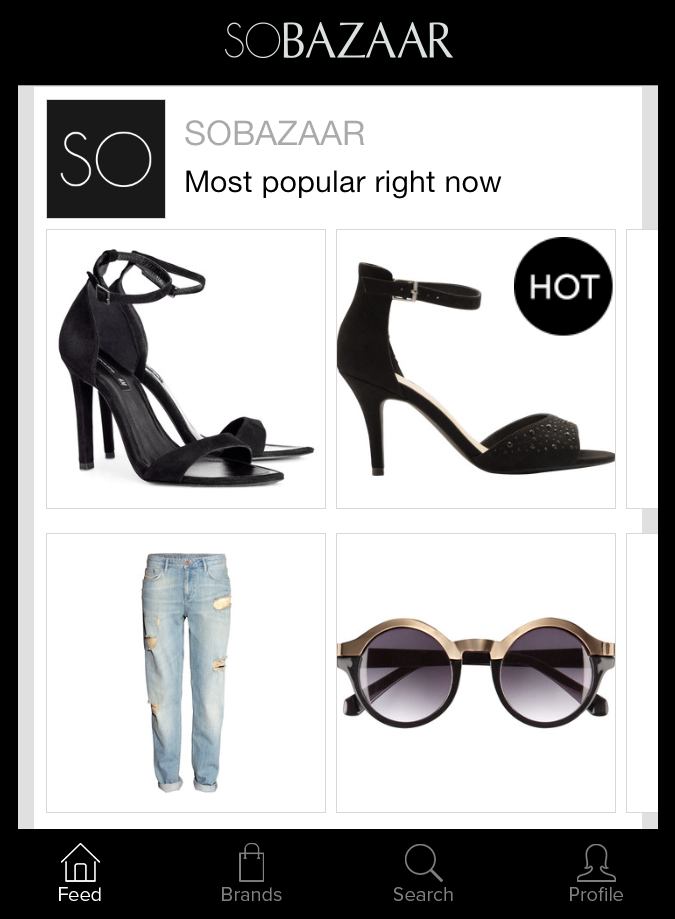
\includegraphics[height=.5\linewidth]{image/SoBazaarmostpop.png}
  \caption[SoBazaar most-popular recommendation]{The Figure shows how the most-popular recommendations are shown in the application}
\label{figure:mostpopular}
\end{figure}

Much like the social feed shown in Figure \ref{figure:SoBazaarfeed} up to 20 popular items can be shown.
It would also be beneficial to rank these recommendations putting the most popular/relevant items in the first 4 slots and sorting the remaining items in descending order based on popularity. This implicates that a metric that measures the overall ranking is not appropriate, and that we only should measure the ranking quality of the $k$ items being shown, the other items are irrelevant. The above reasoning lead us to take a closer look at classification and ranking accuracy metrics.

%TODO - Add some more cites

The area under curve (AUC) is a popular classification accuracy metric. ROC curves provide a graphical
representation for the performance of a recommender system, by plotting the recall (True positive rate)
against the fallout (False positive rate) for increasing recommendation set size. A perfect recommender
would therefore yield a ROC curve that goes straight up towards 1.0 recall and 0.0 fallout until all
relevant items are retrieved. Afterwards it would go straight towards 1.0 fallout while the remaining
irrelevant items follow. One therefore obviously aims to maximize the area under the curve (AUC). The higher
up all relevant items (True positives) are in the recommendation list, the higher the AUC score will be.
AUC can therefore be used as a single measure for the overall quality of a recommender system. Table \ref{table:auc}
shows an example of the AUC values when varying the position of a single relevant document through the
recommendation list.

\begin{table}[H]
	\centering
	\begin{tabular}{*{12}l}
	\toprule
	\#Example	& R1 & R2 & R3 & R4 & R5 & R6 & R7 & R8 & R9 & R10 & AUC \\ \midrule
	1		& \cmark & \xmark & \xmark & \xmark & \xmark & \xmark & \xmark & \xmark & \xmark & \xmark & 1.000 \\ 
	2		& \xmark & \cmark & \xmark & \xmark & \xmark & \xmark & \xmark & \xmark & \xmark & \xmark & 0.889 \\ 
	3		& \xmark & \xmark & \cmark & \xmark & \xmark & \xmark & \xmark & \xmark & \xmark & \xmark & 0.778 \\ 
	4		& \xmark & \xmark & \xmark & \cmark & \xmark & \xmark & \xmark & \xmark & \xmark & \xmark & 0.667 \\ 
	5		& \xmark & \xmark & \xmark & \xmark & \cmark & \xmark & \xmark & \xmark & \xmark & \xmark & 0.556 \\ 
	6		& \xmark & \xmark & \xmark & \xmark & \xmark & \cmark & \xmark & \xmark & \xmark & \xmark & 0.444 \\ 
	7		& \xmark & \xmark & \xmark & \xmark & \xmark & \xmark & \cmark & \xmark & \xmark & \xmark & 0.333 \\ 
	8		& \xmark & \xmark & \xmark & \xmark & \xmark & \xmark & \xmark & \cmark & \xmark & \xmark & 0.222 \\ 
	9		& \xmark & \xmark & \xmark & \xmark & \xmark & \xmark & \xmark & \xmark & \cmark & \xmark & 0.111 \\ 
	10		& \xmark & \xmark & \xmark & \xmark & \xmark & \xmark & \xmark & \xmark & \xmark & \cmark & 0.000 \\
	\bottomrule
	\end{tabular}
	\caption{Varying the position of a single relevant item on a four out of ten recommendation list}
	\label{table:auc}
\end{table}

One should also be aware of that the AUC scores can be highly inaccurate, especially for cold-start users,
users which the recommender is unable to provide more than a handful of recommendations for. This is
due to the fact that all unknown ratings are appended in random order after the known recommendations.
E.g. lets say the recommender is able to generate 10 recommendations for a user out of 4000 items,
and that one out of two test items for that user is not in the recommended list from the recommender.
Where the last test item is appended in the recommendation list can mean the difference between a AUC score of above
0.9 to less than 0.6 if the item is appended at the end of the list, the results can be even more
severe if none of the items is in the initial recommended list, then the results for that user will be completely random. The most obvious solution to this problem would be to use resampling or to repeat
the experiment multiple times where the items not in the recommendation list are drawn at random and
the results averaged over all the trials.

However, a frequently uttered point of criticism is that users are often more interested in the items
at the top of a recommendation list but that the AUC measure is equally affected by swaps at the top
or the bottom. To \emph{complement} AUC, we also wish to measure the rank accuracy, to get a better
overall picture of the systems performance. This means that we want to measure whether or not
highly rated items such as purchases, likes etc. are ranked higher than less relevant items such as clicks,
as having these highly ranked items higher up in the recommendation list aligns with our previously
mentioned financial incentives.

%TODO - What is the "best" rank-accuracy metric?

When using rank accuracy metrics, it is worth knowing whether one is measuring total or partial orderings.
Most rank accuracy metrics (e.g. Kendall's tau and Spearman's rho) compare two total ordering. The problem
with these measures is that we in most cases are not provided with a full ranking of the items as most recommendation
algorithms only generate a partial list of items that are likely to be preferred by a user. The remaining items
would therefore have to be concatenated in random order. The recommendation list can also consist of several
items with similar rating that can appear in varying orders. Therefore, in order to create a full ranking of
the items all preference values for the user have to be known. Since the user can express the same rating for similar
items, the list will again contain groups of items that can appear in arbitrary order. However, the largest problem
is posed by items for which no rating is known. These items could hold an arbitrary place within the ranking.
Again, consider an example where a user e.g. have rated 5 items out of 4000, and the recommender is able to recommend
only 10 items for that user. To measure the rank accuracy we would have to randomly add 3995 items to the users known
preference list and 3990 to the users prediction list. Comparing the order of these lists would not make much sense. The bottom line is that in most cases a rank metric for partial ordering would be more appropriate for comparing recommendation lists that are produced by recommenders to item rankings from known user preferences.

We assume that we can recommend at most $k$ items for each user at a time. It also pays to submit all $k$
recommendations, because we are not penalized for bad guesses. We also assume that the order matters, so it
is better to submit more certain recommendations first, followed by recommendations we are less sure about.
Which means that we basically select the $k$ best candidates in order. To reduce the number of randomness in
the results one could choose to only look at the ranking of the top $k$. However, the problem is that the
likeliness of finding a \emph{hidden} item in e.g. the top 20 recommended items is not very large when one is working
with large item catalogs. The problem then, is how to select the value of $k$. Setting it to low you risk
ending up with many $0.0$ values, and when setting it to high you risk including to many \emph{randomly} concatenated 
ratings in the results.

%MyMediaLite Problems
%	Very few 'remaning items' are appended with a rating of 0.0, how do we determine a cutoff point?

%How certain are we about the order? (Do we look at rank? How much weight should be given...?)

Mean average precision (MAP@k), described in Section \ref{subp:mean_average_precision_map_} is a popular metric for search engines and is applied, for example, to report results at the Text Retrieval Conference (TREC). The main weakness with regard to recommender systems is that it assumes that the user is interested in finding many relevant documents for each query, and does not look at the relevance of the items. Consider the following examples where we have three lists of hidden items and three recommendations lists. All none relevant items are labeled with the item-id $0$.

\begin{table}[H]
\label{table:ap}
\centering
\begin{tabular}{*{4}l}
\toprule
Example 	& 	Actual	& 	Recommended		&	AP@4   \\ \midrule
1			& [1,2,3,4]	&	[1,0,0,0]		&	0.250  \\ 
2			& [1,2,3,4]	&	[2,0,0,0]		&	0.250  \\ 
3			& [1,2,3,4]	&	[3,0,0,0]		&	0.250  \\
\bottomrule
\end{tabular}
\caption{AP@4 Scores}
\end{table}

As you can average precision does not consider the order of the actual item list. We want a way to
reward the recommender for getting the highly ranked items right.

Normalized Discounted Cumulative Gain ($nDCG_{k}$), described in Section \ref{subp:normalized_discounted_cumulative_gain_}
is another metric to measure the rank accuracy. It is based on two main assumptions; (1) Highly relevant items are more useful than marginally relevant ones, (2) The lower the ranked position of a relevant item, the less useful it is for the user, since it is less likely to be \emph{examined}. The maybe most interesting aspect of nDCG is that it contains an utility function $rel_i$. One can replace the original utility function and replace it with a function that is more relevant to the application. Two such examples include:

\begin{itemize}
\item $rel_i = 1/log(i+k)$, where i is the index of the item in the actual sorted rating list, where $k$ is a constant.
\item $rel_i = u(i)$, simply assign the rating of an item as its relevance.
\end{itemize}

For our application we believe it to be beneficial to use the rating of the item as a
relevance score, as we could have multiple items with highly similar ratings (thus the same relevance). When using a low $k$ value for the logarithmic alternative this could mean that the relevance between two almost similarly rated items might end up being disproportionately large. We will also most likely look at the 20 top items, which means that the difference between the lower ranked items will be fairly small, as the logarithmic function converges. A third alternative would be to also use some linear decay function. The following table shows the $nDCG$ score for a set of examples where the function $rel_i = 1/log(i+1)$ is used to assign the relevance score to item $i$ in the sorted list of actual ratings. E.g. item one is assigned a relevance score of $1/(log(2)$ and so on. We hope the following table will give the reader a better idea of how $nDCG$ \emph{works}.

\begin{table}[H]
\label{table:ndcg}
\centering
\begin{tabular}{*{4}l}
\toprule
Example 	& 	Actual					& 	Recommended				&	nDCG 	\\ \midrule
1			& 	[1,2,3,4]				&	[1,0,0,0]				&	0.470   \\ 
2			& 	[1,2,3,4]				&	[2,0,0,0]				&	0.360   \\ 
3			& 	[1,2,3,4]				&	[3,0,0,0]				&	0.330   \\ 
4			& 	[1,2,3,4,5,6,7,8,9,10] 	& 	[1,2,3,4,5,6,7,8,9,10] 	&   1.000	\\ 
5			& 	[1,2,3,4,5,6,7,8,9,10] 	& 	[10,9,8,7,6,5,4,3,2,1] 	&   0.900	\\ 
6			&	[1,2,3,4,5,6,7,8,9,10] 	& 	[1,2,0,0,0,0,0,0,0,0] 	&   0.440	\\ 
7			& 	[1,2,3,4,5,6,7,8,9,10] 	& 	[1,0,0,3,0,0,0,0,0,0] 	&   0.390	\\ 
8			& 	[1,2,3,4,5,6,7,8,9,10] 	& 	[4,0,0,0,8,0,0,0,0,0] 	&   0.280	\\ 
9			& 	[1,2,3,4,5,6,7,8,9,10] 	& 	[0,0,0,0,5,0,0,0,0,10] 	&   0.130	\\ 
10			& 	[1,2,3,4,5,6,7,8,9,10] 	& 	[0,0,0,0,0,0,0,0,9,10]	&   0.110	\\
\bottomrule
\end{tabular}
\caption{nDCG Test Examples}
\end{table}

As you can see from the above mentioned examples nDCG will give us an indication whether or not our recommender
ranks \emph{highly relevant} items above those who are less relevant. As for the limitations, nDCG is designed for situations of non-binary notions of relevance, thus it cannot be used in our experiment where we wish to compare binary ratings with implicit ratings. The main difficulty encountered in using nDCG is the unavailability of an ideal ordering of results when only partial relevance feedback is available. This is often the case when we have several equally good results. This is especially true when the metric is limited to only first few results as it is often done in practice.

We chose take a closer look at the different ways of calculating nDCG. There are two commonly used methods used to calculate the DCG and IDCG scores.

\begin{itemize}
\item Method 1  $DCG_p = rel_1 + \sum_{i=2}^{p} \frac{rel_i}{log_2(i)}$
\item Method 2: $DCG_p = \sum_{i=1}^{p} \frac{2^{rel_i}-1}{log_2(i+1})$
\end{itemize}

The following table shows the differences between Method 1 and Method 2 on a few selected examples. Here we set the value of $rel_i$ equal to the implicit rating of item $i$.

\begin{table}[H]
\label{table:ndcgfinal}
\centering
\begin{tabular}{*{5}l}
\toprule
\#Ex & 	Actual																	& 	Recommended				&	$nDCG^1$  	   & $nDCG^2$	\\ \midrule
1 		& 	[$1_{5}, 2_{3.8}, 3_{3.55}, 4_{2.78},5_{1.3}$]								&	[5,0,0,0,0]				&	0.113 		   & 0.026  \\ 
2 		& 	[$1_{5}, 2_{3.8}, 3_{3.55}, 4_{2.78},5_{1.3}$]								&	[0,0,1,0,0]				&	0.217 		   & 0.275   \\ 
3   	& 	[$1_{5},2_{4.8}, 3_{3.55}, 4_{2.78}, 5_{2.2}, 6_{2.0},7_{1.77},8_{1.3}$]		&	[2,3,4,5,6,7,8,0]		&	0.827		   & 0.682   \\ 
4  		& 	[$1_{5},2_{4.8}, 3_{3.55}, 4_{2.78}, 5_{2.2}, 6_{2.0},7_{1.77},8_{1.3}$]		&	[1,2,0,0,0,0,0,0]		&	0.592 		   & 0.805   \\
5 		& 	[$1_{5},2_{4.93},3_{2.88}, 4_{1.85},5_{1.8},6_{1.77}, 7_{1.63},8_{1.52}$]	&	[1,0,0,0,0,0,0,0]		&	0.394 		   & 0.544   \\
6 		& 	[$1_{5},2_{4.93},3_{2.88}, 4_{1.85},5_{1.8},6_{1.77}, 7_{1.63},8_{1.52}$]	&	[3,4,5,6,7,8,0,0]		&	0.542 		   & 0.206   \\
\bottomrule
\end{tabular}
\caption{Comparison of nDCG scores for different methods of computing DCG. Each item in the Actual list is on the form $ItemId_{Rating}$, the first item in the actual list of example one therefore has en ItemId of 1 and a Rating of 5. All non relevant items are given the ItemId 0 in the Recommended list.}
\end{table}

As you can see Method 1 is a bit more \emph{balanced} than Method 2, as it does not give as much weight to highly rated items. Especially example 5 and 6 highlights this as Method 2 prefers retrieving one highly rated item over retrieving multiple less relevant ones. Method 2 is ultimately closer to what we want in addition to being commonly used by web search companies and on the data science competition platform Kaggle \cite{kaggle}. We have also chosen to truncate the recommendation list and only calculate the nDCG of the $k$ top items. Because nDCG has a relatively low positional discount, it allows us to set $k$ fairly high, but this only makes sense if we believe that the user will read large portions of the recommendation list. 

\marginpar{TODO: Spend any more time looking at partial order ranking measures?...}

%TODO - Select K value based on user interface
%TODO - Justify why these metrics combined will give a good overview of the performance.
%TODO - Cold-start evaluation Metrics

In addition to looking at the above mentioned metrics it would be interesting to see how
the different sparsity levels affect both the user- and item-space coverage of the different
methods when evaluating the cold-start system performance, as having a recommender that can only
recommend a limited set of items to a small portion of the users is \emph{unfortunate}. The
user-space coverage is the number of users the recommender is able to produce recommendations for while the item-space
coverage is measured by looking at how many of the items are recommendable.

%TODO - How will these experiment be carried out and validated?

\subsection{Comparing ratings}

Figure \ref{implicitRatingEvaluation} shows the process of evaluating a set of generated ratings. The \emph{million dollar question} is: how to do we evaluate a set of ratings?

\begin{figure}[H]
		\centering
	  	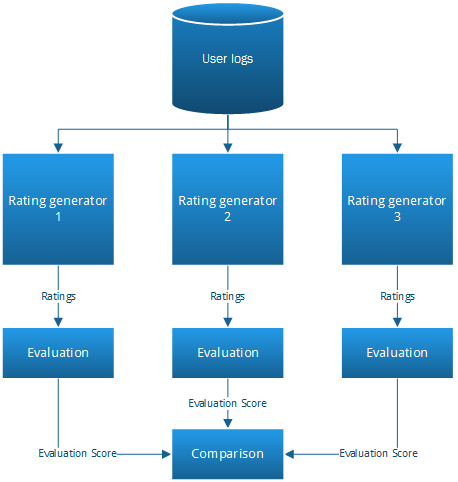
\includegraphics[height=0.65\linewidth]{image/ratinggeneval.png}
		\caption[Comparing Ratings]{The Figure shows the process of comparing ratings}
		\label{figure:compareratings}
\end{figure}

Evaluating and comparing a set of ratings is not something you often encounter in the literature.
\marginpar{TODO: Are there any articles on something similar?}
We have a few initial theories of how it can be done:

\begin{enumerate}
\item Using the log data as the ground truth. Is it possible to justify that one method is better than another with observations from the log data?
\item Can we put the ratings into a traditional recommender system evaluation pipeline and use the results from that to compare the ratings. In that case, what evaluation metrics are suitable?
\end{enumerate}

The bottom line is that evaluating the quality of a set of generated ratings is hard. 



We could say that we believe that better ratings gives us better recommendation results, and use this as a basis for our evaluation. However, this means that the results we get from testing the different algorithms with different rating sets should be comparable. The problem with this is that most evaluation metrics consider the supplied ratings as the ground truth and bases its evaluation on these numbers. This automatically disqualifies any evaluation metrics that consider the rating values such as e.g. MAE.


\subsection{Implicit Ratings vs. Binary Preference}

This subsection will attempt to explain how we will attempt to determine whether our implicit gives some added
qualities in form of improved recommendations produced using binary preferences.

Problems: Methods that can incorporate both types of feedback...
Problems: Methods for implicit ratings (Explain why traditional item-based cf is not suited...)

\begin{center}
    \begin{tikzpicture}
		[node distance = 1cm, auto,font=\footnotesize,
		% STYLES
		every node/.style={node distance=1.5cm},
		% The comment style is used to describe the characteristics of each process
		comment/.style={rectangle, inner sep= 5pt, text width=3cm, node distance=0.25cm, font=\scriptsize\sffamily},
		% small comment lol
		comment-small/.style={rectangle, inner sep= 5pt, text width=1cm, node distance=0.25cm, font=\scriptsize\sffamily},
		% The nonProcess style
		nonProcess/.style={rectangle, draw, inner sep=5pt, text width=3cm, text badly centered, minimum height=1.2cm, font=\footnotesize\sffamily},
		% The process style is used to draw the processs' name
		process/.style={rectangle, draw, fill=black!10, inner sep=5pt, text width=3cm, text badly centered, minimum height=1.2cm, font=\bfseries\footnotesize\sffamily},
		% ratingsGenerator style
		ratingsGenerators/.style={rectangle, draw, fill=blue!50, inner sep=5pt, text width=3cm, text badly centered, minimum height=1.2cm, font=\bfseries\footnotesize\sffamily},
		% racommendation algorithms
		recAlgs/.style={rectangle, draw, fill=red!40, inner sep=5pt, text width=3cm, text badly centered, minimum height=1.2cm, font=\bfseries\footnotesize\sffamily}]

		% Draw processs
		\node [ratingsGenerators] (rg1) {sigmoid\_fixed};
		\node [ratingsGenerators, right=0.25 of rg1] (rg2) {sigmoid\_constant};
		\node [comment-small, right=0.01 of rg2] (dotdotdot) {..............};
		\node [ratingsGenerators, right=0.01 of dotdotdot] (rg3) {norm\_dist};

		\node [process, below of=rg2] (gt) {"Ground Truth"};

		\node [recAlgs, below of=gt] (ra2) {ALS};
		\node [recAlgs, left=0.25 of ra2] (ra1) {KNN};
		\node [comment-small, right=0.01 of ra2] (dotdotdot2) {..............};
		\node [recAlgs, right=0.01 of dotdotdot2] (ra3) {wALS};

		\node [process, below of=ra2] (eval) {Evaluation Score};

		% \node [nonProcess, below of=implicitConverter] (ratings) {Ratings for the items};
		% \node [process, below of=ratings] (recommendations) {Make recommendations};
		% \node [process, below of=recommendations] (evaluations) {Evaluate recommendations};
		% \node [nonProcess, below of=evaluations] (evaluationValue) {Recommendation score};

		%%%%%%%%%%%%%%%
		% Comments
		\node [comment, right=0.25 of rg3] (comment-rg3) {
			Implicit ratings
		};
		\node [comment, right=0.25 of ra3] (comment-ra3) {
			Recommendations algorithm
		};
		% \node [comment, right=0.25 of ratings] (comment-ratings) {
		% The output of the conversion is a set of ratings on the different items from the SoBazaar dataset
		% };
		% \node [comment, right=0.25 of recommendations] (comment-recommendations) {
		% Makes recommendations based on the inputed ratings. Different approaches to make the recommendations can be take, such as matrix factorization or neighborhood based approaches
		% };
		% \node [comment, right=0.25 of evaluations] (comment-evaluations) {
		% Evaluate the recommender system(s). Different evaluation metrics will be usea, such as e.g. AUC and nDCG
		% };

		%%%%%%%%%%%%%%%%
		% Draw the links between processs
		\path[->,thick]
			(rg1) edge (gt)
			(rg2) edge (gt)
			(dotdotdot) edge (gt)
			(rg3) edge (gt)
			(gt) edge (ra1)
			(gt) edge (ra2)
			(gt) edge (dotdotdot2)
			(gt) edge (ra3)
			(ra1) edge (eval)
			(ra2) edge (eval)
			(dotdotdot2) edge (eval)
			(ra3) edge (eval);
		% \path[>=latex,->] (gt) edge (eval);
		% \draw[rectangle connector=-3cm] (gt) to (eval);
		\draw[>=latex,->] (gt) -- +(-6,0) |- (eval);
    \end{tikzpicture}
    \captionof{figure}[Implicit Rating Evaluation]{Overview of how the generated ratings from the implicit feedback can be evaluated.}
  	\label{figure:implicitRatingEvaluation}
  \end{center}

The blue boxes in figure~\ref{figure:implicitRatingEvaluation} are functions used to produce the implicit ratings based on the implicit feedback. Based on this, the system gets an estimated \emph{ground truth}, which can be used to evaluate the different recommendation algorithms show in the red boxes. Based on the evaluation score something can be said about the implicit feedback conversion to implicit ratings and the recommendation algorithms used.


\subsection{A Comparison of Implicit Rating Mapping Functions}



\subsection{Combining Implicit Ratings With Existing Cold-Start Solutions}


Only use cold-start splits for this sections tables.

Comparison of recency functions in filterbots?
E.g. does the PopularityBot perform better when only considering the last x weeks or all the data?
Similarly for the criticBot


